\section{Methodology}

\subsection{Knowledge Graph Design and Construction}

One of the main challenges and core components of this project was designing and populating the knowledge graph that would be used to train the recommendation algorithm. To support this objective, the knowledge graph had to be designed carefully to accommodate both diverse musical attributes and user behavior, as well as the relational structure necessary for effective representation learning.

The knowledge graph was built on top of an existing music ontology \cite{raimond2007musicontology}, with classes and properties tailored to music recommendation systems. Standard vocabularies expressed in RDF such as FOAF for agents, or event ontology for listening events were reused to ensure that the graph is interoperable with other Semantic Web tools and that its structure is transparent to readers familiar with these standards. A small number of project-specific relations were added under a dedicated \textit{mrc:} namespace to cover concepts not present in the existing vocabularies, such as the link between a \textit{performance} and its \textit{tempo} category, or between a \textit{listening} event and its play count.

\subsubsection{Simple Knowledge Graph}

The knowledge graph was built from accurately matched tracks described by both MSD metadata and successfully extracted musical features. Not all metadata fields available in the merged dataset were retained for the graph, but rather only those mapping onto a meaningful concept within the ontology. The features were carefully selected to ensure that every retained field could be expressed as either a node, an edge, or an interpretable property within the ontology (e.g. artist and track identifiers, title, album, release year, genre tags, or MIDI instrumentation). Derived audio descriptors such as danceability and energy, or popularity scores were excluded from the graph but remained available in the underlying tabular dataset for use in the subsequent modeling and evaluation stages, ensuring that the graph contains only information that contributes to the relational structure used by the recommender. Out of 40 columns produced by the MSD-Lakh integration, only 22 were kept for the KG. 

Similarly, out of the 1,525 musical features extracted per track, 11 were incorporated into the graph as datatype properties on the corresponding Track node (e.g., mrc:meanTempo, mrc:noteDensity). All selected features represented a single, well-defined musical attribute such as mean tempo, note density, amount of staccato, or average number of independent voices. Most of the remaining musical features almost entirely consisted of multi-bin histograms such as pitch, melodic interval, beat, rhythmic value, or instrument-prevalence histograms, whose individual bins did not correspond to musically meaningful concepts, therefore they were excluded from direct representation. Importantly, the selection was not based on a systematic ranking of feature importance, but rather served as an illustrative demonstration of how symbolic music features can be represented within an OWL ontology. The remaining musical features, while musically interpretable, were retained in tabular form and fed in their entirety to the autoencoder, whose compressed output served as the track node feature in the GNN. This decision was made because including these features would clutter the graph without contributing much usable relational information.

The complete list of features included in the knowledge graph, along with their descriptions, origins, and corresponding RDF mappings, is provided in Table~\ref{tab:kg_features} in the Appendix.

In the knowledge graph, each row of the merged dataset translates to a connected cluster of nodes representing the entities associated with that recording. Categorical and relational concepts such as genres, instruments, musical keys, modes, and tempo classes were encoded as named individual nodes reused across tracks, enabling the graph to capture shared structure between recordings. Continuous scalar measurements, unique to each track such as tempo, note density, or loudness were, on the other hand, encoded as datatype literals attached to the corresponding track or performance node. 

Core node types follow the Music Ontology design: a \textit{Track} carries bibliographic metadata and 11 musical datatype properties (e.g.\ note density, chromatic motion); an \textit{Artist} links to a \textit{Performance} node that stores tempo and bridges to one of nine categorical \textit{TempoClass} individuals (e.g.\ Andante, Allegro) and one or more \textit{Instrument} nodes from the MIDI file. Tonal properties---\textit{Key} (12 chromatic values) and \textit{Mode} (Major/Minor)---point to shared named individuals rather than per-track literals, enabling cross-track joins in SPARQL. \textit{Genre} nodes are attached at the artist level and likewise reused across all artists sharing the same tag.

The ontology was further enriched by aligning core classes to the Wikidata upper-concept hierarchy via OWL semantics: \texttt{mrc:Genre}~$\equiv$~\texttt{wd:Q188451}, \texttt{mo:Instrument}~$\equiv$~\texttt{wd:Q34379}, and \texttt{mrc:Key}~$\equiv$~\texttt{wd:Q534932}, with the two mode individuals additionally grounded via \texttt{owl:sameAs}. This positions genre, instrument, key, and tempo class within a universally recognised framework, and the shared named individuals create cross-track bridges that let GNN message passing propagate musical context across otherwise disconnected graph regions. Only English labels were retained, as they provided complete coverage across all aligned Wikidata entities.

Release years were bucketed into decade nodes (1960s--2010s), linked into a temporal sequence via \texttt{wdt:P155}/\texttt{wdt:P156} and grounded to their Wikidata decade entities. This converts a sparse scalar into a shared structural node that hundreds of tracks can co-reference, making the temporal signal exploitable by both SPARQL and GNN message passing.

Finally, the behavioural layer from the Echo Nest Taste Profile was added: each unique user becomes an \texttt{mrc:Listener} node (\texttt{foaf:Agent} subclass) and each interaction a direct \texttt{mrc:listenedTo} edge to the matched track, retaining only rows whose \texttt{song\_id} already existed in the graph.

A summary of user-related graph components introduced in the behavioral layer is available in Table~\ref{tab:taste_profile_features} of the Appendix.

\subsubsection{Rich version of the Knowledge Graph}

On the top of the presented knowledge graph, a second, richer version of it was additionally created that preserves extra details such as weights, counts, and confidence, preserving all the information from the source dataset. This version matches the Music Ontology's intended modeling much more closely, and allows for more advanced SPARQL inspection and qualitative evaluation, using KG embedding methods that can handle heterogeneous edges, and for frequency-aware recommendation. 

In this version, genre associations are reified as blank nodes of type mrc:GenreAssociation, each carrying an mrc:weight value representing the strength of the genre tag, taken either from MSD's published artist\_terms\_weight or, when missing, from a rank-based fallback. Key and mode are attached to a mo:Performance node rather than directly to the Track, and additionally carry confidence scores (mrc:keyConfidence, mrc:modeConfidence), creating a conceptually cleaner separation and allowing the certainty of the audio analysis to be represented explicitly. Lastly, the listen count is stored as a property of a mrc:ListeningEvent blank node, allowing the model to treat repeated listening as a stronger preference signal than a single play.

Differences between the simple and rich knowledge graph representations in details are represented in Table ~\ref{tab:simple_vs_rich} of the Appendix.

Because the rich variant encodes genre associations and listening events as blank nodes, it was primarily constructed for ontological demonstration and SPARQL inspection in GraphDB rather than as a direct model input. The recommendation model uses the topological structure of the simple KG, extended with edge attributes for relational weights, while all 1,525 musical features are injected via the autoencoder as track node features.

\subsection{TBox representation}

\begin{figure}[H]
    \centering
    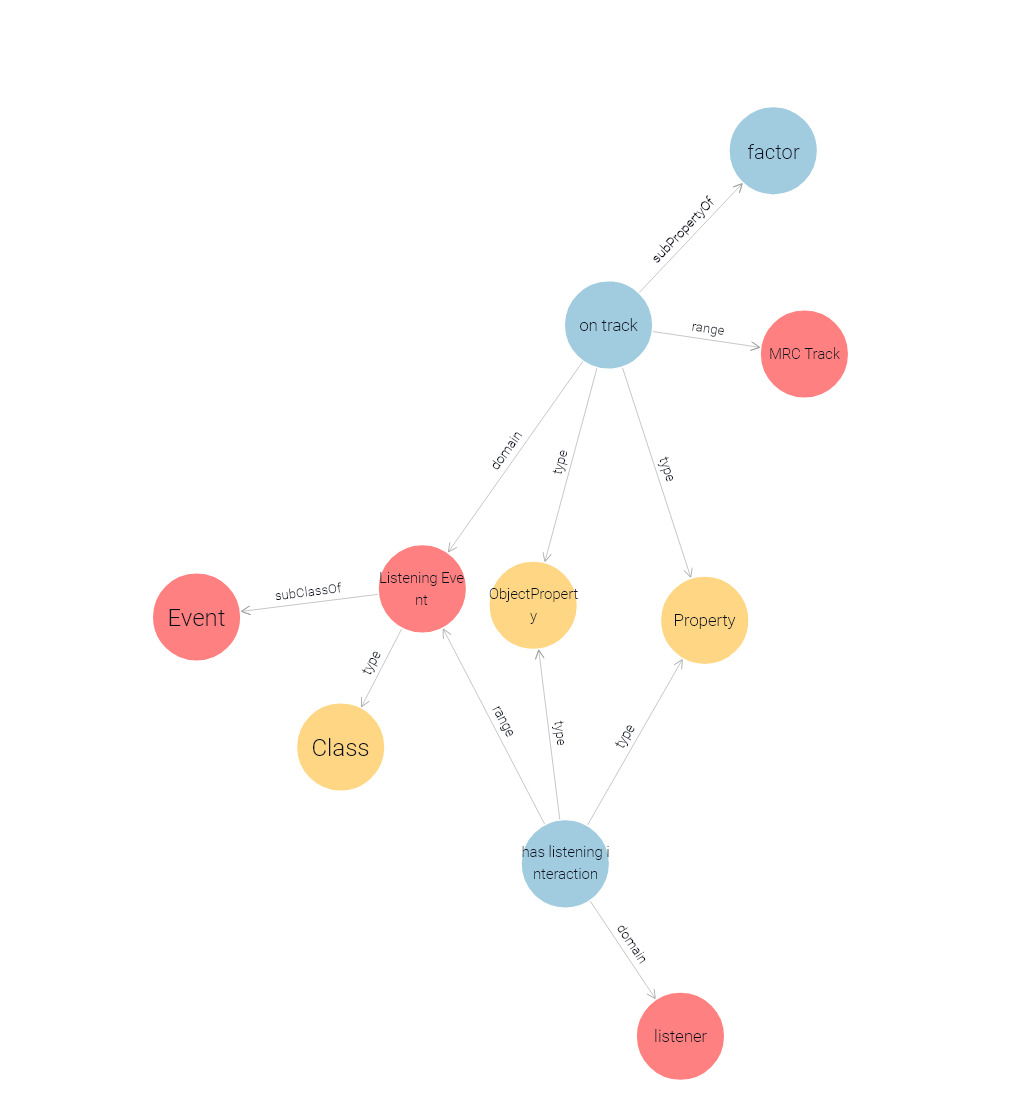
\includegraphics[width=0.75\linewidth]{sec/graph_DB/TBox.jpeg}
    \caption{TBox fragment showing the schema-level definition of \texttt{mrc:ListeningEvent} and its connecting properties in GraphDB.}
    \label{fig:TBox}
\end{figure}

Figure~\ref{fig:TBox} shows a fragment of the TBox, illustrating how user listening behaviour is modelled at the schema level. The class \texttt{mrc:ListeningEvent} is declared as a subclass of \texttt{mo:Event} from the Music Ontology, grounding the vocabulary in an established standard. Two object properties govern its connectivity: \texttt{mrc:hasListeningInteraction}, with domain \texttt{mrc:Listener} and range \texttt{mrc:ListeningEvent}, links a user to their listening events; and \texttt{mrc:onTrack}, with domain \texttt{mrc:ListeningEvent} and range \texttt{mrc:MSDTrack}, associates each event with the track that was played. The latter is further declared a sub-property of \texttt{mrc:factor}, reflecting its role as a contributing signal in the recommendation context. 


\subsubsection{Semantic Inspection}

Both KG variants were loaded into GraphDB and validated through SPARQL queries covering genre rankings, confidence-filtered key distributions, ontological hierarchy traversals, the decade temporal chain, and top-listened track lookups. Results are reported in Section~\ref{sec:formatting} and query listings are provided in the Appendix.



\subsection{From Knowledge Graph to Learnable Tensors}

Before any neural model could consume the graph, the RDF triples were converted
into a typed tensor representation. A dedicated extraction routine streamed the
graph into (i)~a consolidated triple table and an edge dictionary, and
(ii)~a heterogeneous \texttt{PyTorch~Geometric} graph in which every ontology
class becomes a distinct node type (\texttt{user}, \texttt{track},
\texttt{artist}, \texttt{genre}, \texttt{instrument}, \texttt{key},
\texttt{mode}, \texttt{tempoClass}, \texttt{decade}) and every predicate is a
typed relation. Track nodes were initialised with the content embeddings
produced by the autoencoder described below, and the remaining node types received
either knowledge-graph-embedding features or learnable lookup vectors. Because
the listening layer of the simple graph encodes each interaction as a direct
\texttt{user\,$\rightarrow$\,track} edge, message passing can reach items in a
single hop, which is the configuration used to train the main recommender.


\subsection{Representation Learning and Recommendation Models}

We trained three representation/recommendation components on top of the music knowledge graph, and compared them against three baselines on a shared, stratified user-level interaction split.

\subsubsection{Symbolic-feature autoencoder}

Because the remaining jSymbolic features per track were too high dimensionally and noisy to use them directly as node features in the GNN, an autoencoder was used to reduce them to a compact, dense representation that still preserves the most important musical structure.

The full 1{,}526-dimensional jSymbolic vector of each track was standardised and passed through a fully connected autoencoder with encoder $1526\!\rightarrow\!512\!\rightarrow\!256\!\rightarrow\!128$ and a symmetric decoder ($128\!\rightarrow\!256\!\rightarrow\!512\!\rightarrow\!1526$), and with each layer followed by ReLU activation and dropout~0.2. Training used Adam (learning rate $10^{-3}$, batch size~256) to minimise mean-squared reconstruction error, with up to 200 epochs and early stopping once the training loss fails to improve by more than $10^{-4}$ for 15 consecutive epochs. Because the task was pure transductive compression of a fixed catalogue, no held-out ranking split was required. The 128-dimensional bottleneck was exported as a dense content embedding for every track and used both to initialise the track node features of the graph models and as the item representation of the hybrid baseline.

\subsubsection{Knowledge-graph embeddings.}

Because our KG contains many node types that don't have numeric features from any source, a numeric representation that could be used as input features for the GNN was required. This numeric representation was achieved by training  KG embedding models that learn a dense vector for every entity in the graph purely from the graph's relational structure.

Two KG embedding models were trained on triples exported from the enriched KG. RotatE~\cite{sun2019rotate}, which represents each entity as a complex vector and each relation as a rotation in complex space, and ComplEx~\cite{trouillon2016complex}, which uses a similar complex-valued representation but scores triples via the real part of a three-way interaction between head, relation, and tail entities. Both being well-established complex-valued KGE models that can handle diverse relation types well.

Both models were chosen because our KG is rich in \emph{asymmetric} relations: a user listens to a track but not the reverse; a track belongs to a genre but a genre does not belong to a track; an artist performs a piece but a piece does not perform an artist. Real-valued models such as TransE cannot represent asymmetry, since they place head and tail in the same vector space with a single additive offset that is the same in both directions. Complex-valued representations break this symmetry naturally: in RotatE, a relation $r$ rotates the head entity $h$ to reach the tail $t$ in complex space ($h \circ r \approx t$, element-wise), but the inverse rotation $\bar{r}$ is a distinct transformation, so the model can simultaneously encode $r$ and its asymmetric inverse without conflict. ComplEx achieves asymmetry through the Hermitian dot product $\mathrm{Re}(\langle h, r, \bar{t}\rangle)$, where conjugating $t$ but not $h$ breaks the symmetry of the score.

Despite sharing the complex-space inductive bias, RotatE is expected to be the stronger embedding for this KG due to its ability to model \emph{compositional} relation patterns in addition to symmetry and antisymmetry. Composition arises naturally in our graph: the chain \textit{track~$\xrightarrow{\text{hasTempoClass}}$~Allegro~$\xrightarrow{\text{followedBy}}$~decade} or genre-hierarchy traversals are all compositional paths. A rotation composed with another rotation is still a rotation, so RotatE can represent such chains geometrically; ComplEx has no analogous closure property and therefore struggles to encode compositional structure. For these reasons RotatE was used as the primary initialiser for the HGT node features, with ComplEx retained for comparison.

Both KG embeddings were trained with entity\_dim=128, producing 256-dimensional output vectors per entity, over 100 epochs with Adam optimizer, and with listening events deliberately excluded from the training corpus. The embedding dimension was set to 128 to match the autoencoder bottleneck, ensuring that audio and structural features contribute comparably to the final track representation. Listening interactions, on the other hand, were excluded from the training corpus to avoid leaking the target signal into the node features.

The resulting 256-dimensional embedding for every entity in the graph, were subsequently used to initialise node features for all node types in the graph.

\subsubsection{Heterogeneous Graph Transformer (The main model).}

The primary recommendation model used in this project was a Heterogeneous Graph Transformer (HGT)~\cite{hu2020hgt}, selected for its ability to natively operate on graphs containing multiple node and edge types. This was particularly important for our KG since it comprises tracks, artists, users, genres, instruments, keys, modes, tempos, and decades, each representing distinct semantic entities and relationships. Many standard graph neural network architectures aggregate information from neighbouring nodes without explicitly modelling these type differences, potentially obscuring important structural information. In contrast, HGT learns type-specific transformation and attention parameters for each node and edge type combination, enabling it to preserve the heterogeneous structure of the graph throughout the message-passing process and capture more nuanced relationships for recommendation, making it a natural fit for this task. 

The HGT stack was configured with two message-passing layers, 4 attention heads, a hidden dimension of 128, and dropout of 0.1. A per-node-type MLP head projects the hidden representations to a 64-dimensional output space, which is L2-normalised to enable cosine similarity scoring, a standard output design for dot-product recommenders. Track nodes were initialised with a 384-dimensional feature vector, the concatenation of the 128-dim autoencoder embedding and the 256-dim KGE embedding, giving the model access to both audio content and relational context. All other node types (artists, genres, instruments, keys, modes, tempos, decades) were initialised from their 256-dim KGE features alone.

The model was trained for 100 epochs using the Adam optimiser
($lr = 10^{-3}$, weight decay $=10^{-4}$) with a cosine
warm-restart learning-rate schedule that periodically reset the
learning rate to escape local minima. The checkpoint achieving the best validation Recall@20 was retained for final evaluation.

To address the popularity bias inherent in implicit-feedback data, we adopt an \textit{Intensity-Weighted Listwise Loss with Logit Adjustment}. Given $L_2$-normalised user embedding $\hat{\mathbf{u}}$ and track embeddings $\hat{\mathbf{t}}_i$, the adjusted logit for track $i$ is
\begin{equation}
s_i = \tfrac{\hat{\mathbf{u}}^\top \hat{\mathbf{t}}_i}{\tau} + \lambda \log p_i,
\end{equation}
where $\tau{=}0.1$ sharpens the softmax distribution and $p_i$ is the Laplace-smoothed marginal listen probability of track $i$. Since $\log p_i < 0$, popular tracks receive a downward logit adjustment and less-heard items are relatively boosted, directly discouraging the model from concentrating recommendations on globally popular choices.

Soft training targets per user are constructed from raw play counts as $\tilde{p}_{ui} \propto \log(1+c_{ui})$, normalised row-wise to a valid probability distribution. The log-transform compresses the count range so that repeat listening contributes a stronger but diminishing signal. The loss is then the cross-entropy between the adjusted softmax and the soft target distribution, averaged over the user batch:
\begin{equation}
\mathcal{L} = -\frac{1}{|B|}\sum_{u\in B}\sum_i \tilde{p}_{ui}\,\log\mathrm{softmax}(\mathbf{s}_u)_i.
\end{equation}

This formulation was chosen over binary cross-entropy or BPR because: (i)~the listwise objective ranks across the full catalogue simultaneously; (ii)~logit adjustment counters the popularity shortcut without heuristic negative sampling; and (iii)~soft engagement-weighted targets exploit the ordinal information in play counts. At inference, items are ranked by cosine similarity with training-seen items masked.


\subsubsection{Baselines}
Three baselines were used to contextualise the performance of the graph-based model, each representing a different level of complexity and a different source of signal.

The first baseline, MostPopular, ranks all unseen items by global play frequency and recommends the most-played tracks to every user identically, serving as a lower bound that any useful recommender should outperform it.

The second baseline, KNN-CF, is a user–user collaborative filter operating on the $\ell$2-normalised interaction matrix, where similarity between users is measured by cosine distance. For each user, item scores were aggregated from the k most similar neighbours, and unseen items were ranked by this aggregate. The neighbourhood size k was selected via a sweep over candidate values, choosing the k that maximised a composite validation score. This baseline captured behavioural similarity between users without any content or graph information, isolating the contribution of interaction patterns alone.
The third baseline, an XGBoost two-stage hybrid, incorporates content features without graph structure. Top-200 candidates per user were retrieved via cosine similarity between a mean-pooled autoencoder user profile and track content embeddings, then re-ranked with a gradient-boosted learning-to-rank model (\texttt{rank:ndcg@10}, up to 300 rounds, early stopping at 30) trained on 3{,}000 sampled users. The 300-dimensional feature vector per (user, track) pair concatenated the 128-dim user-profile and track-AE embeddings with 44 categorical features (one-hot key/mode/tempo class, target-encoded genre and artist, multi-hot instrument indicator). This hybrid fuses content and behaviour without graph structure, directly isolating the GNN's contribution.

\subsubsection{Evaluation Protocol}

All recommenders were evaluated on a single, shared \emph{user-level stratified}
split of the interaction data (training / validation / test), stratified by
song-level attributes (genre and release decade) so that the popularity and
content distributions were preserved across folds; song features and graph
structure were visible to every split, and only the interactions were
partitioned, preventing leakage. Knowledge-graph embeddings and the autoencoder
are unsupervised and therefore fit on the training data without a held-out
ranking split.

We report a standard top-$K$ suite---Recall@$K$, Precision@$K$, NDCG@$K$, Hit-Rate@$K$ and MRR---together with two catalogue \emph{Coverage} and mean \emph{Popularity-Bias@$K$}, and a composite \emph{Overall Score}
\begin{multline}
\mathrm{Overall} = 0.6\cdot\mathrm{NDCG@}K + 0.2\cdot\mathrm{Coverage} \\
+ 0.2\cdot(1-\mathrm{PopularityBias@}K),
\end{multline}
which rewards models that are accurate \emph{and} surface diverse, less
popular content. Every model was scored with the same recommendation lists sliced at
$K\in\{5,10,20,50,100\}$. Pairwise differences were assessed with the
paired Wilcoxon signed-rank test (with Cohen's~$d_z$ effect sizes) and an
omnibus Friedman test. Because full inference over all 284{,}864 test users
is computationally prohibitive for the XGBoost model, pairwise and omnibus
tests were conducted on a shared random subsample of 5{,}000 users across all
models, ensuring a balanced, paired comparison.

